\chapter{Dirac-Gleichung in der T0-Theorie: \\
	Geometrische Integration mit Zeit-Masse-Dualität \\
	\large Fraktale Raumzeit und dynamische Masse}

	
	
\section*{Abstract}
		Diese Arbeit integriert die Dirac-Gleichung vollständig in das T0-Theorie-Rahmenwerk. 
		Im Gegensatz zur Standard-Formulierung mit konstanter Masse verwendet die T0-Theorie 
		die fundamentale Zeit-Masse-Dualität $T(x) \cdot m(x) = 1$, was zu einer 
		raumzeit-abhängigen Masse führt. Die fraktale Dimension $D_f = 3 - \xi$ modifiziert 
		die zugrunde liegende Metrik und damit den Differentialoperator. Wir zeigen, wie 
		die Clifford-Algebra-Struktur natürlich mit der Torus-Topologie der T0-Theorie 
		verbunden ist und wie Spin-1/2 als topologische Wicklungszahl interpretiert werden 
		kann. Die Vorhersagen werden als verhältnisbasierte Aussagen formuliert, die 
		unabhängig von Einheitensystemen und phänomenologischen Parametern sind. 
		Experimentelle Tests bei Belle II können die fundamentale quadratische 
		Massenskalierung direkt überprüfen.

	
	
	\section{Einführung: T0-Grundprinzipien}
	
	\subsection{Zeit-Masse-Dualität}
	
	Das fundamentale Prinzip der T0-Theorie ist die Zeit-Masse-Dualität:
	
	\begin{equation}
		T(x,t) \cdot m(x,t) = \frac{\hbar}{c^2}
		\label{eq:time_mass_duality}
	\end{equation}
	
	In natürlichen Einheiten ($\hbar = c = 1$):
	\begin{equation}
		T(x,t) \cdot m(x,t) = 1
		\label{eq:tmd_natural}
	\end{equation}
	
	Dies bedeutet: **Die Masse ist nicht konstant, sondern ein dynamisches Feld**, 
	gekoppelt an das intrinsische Zeitfeld $T(x,t)$.
	
	\subsection{Fraktale Raumzeit}
	
	Die T0-Theorie postuliert eine fraktale Raumzeit-Dimension:
	\begin{equation}
		D_f = 3 - \xi \quad \text{mit} \quad \xi = \frac{4}{3 \times 10^4} \approx 1.333 \times 10^{-4}
		\label{eq:fractal_dim}
	\end{equation}
	
	Diese modifiziert die Metrik und damit alle Differentialoperatoren.
	
	\subsection{Torus-Topologie}
	
	Die zugrunde liegende Topologie ist ein Torus mit charakteristischen Skalen:
	\begin{itemize}
		\item Großer Radius: $R \sim 1/\xi$
		\item Kleiner Radius: $r \sim R \cdot \xi$
		\item Wicklungszahlen: $(n_\theta, n_\phi)$ für poloidale und toroidale Richtung
	\end{itemize}
	
	\section{Standard-Dirac-Gleichung: Probleme}
	
	\subsection{Die Standard-Form}
	
	Die übliche Dirac-Gleichung lautet:
	\begin{equation}
		(i\gamma^\mu \partial_\mu - m)\psi = 0
		\label{eq:standard_dirac}
	\end{equation}
	
	mit konstanter Masse $m$ und flacher Minkowski-Metrik.
	
	\subsection{Probleme für die T0-Integration}
	
	\begin{enumerate}
		\item \textbf{Konstante Masse:} Widerspricht der Zeit-Masse-Dualität
		\item \textbf{Flache Metrik:} Ignoriert die fraktale Struktur
		\item \textbf{Keine Topologie:} Spin hat keinen geometrischen Ursprung
		\item \textbf{Statisch:} Keine Kopplung an Zeitfeld
	\end{enumerate}
% DIESES KAPITEL EINFÜGEN IN 051_dirac_De_v2.pdf
% NACH SECTION 2.2 (Probleme für die T0-Integration)
% VOR SECTION 3 (T0-Dirac-Gleichung: Geometrische Form)

\section{Clifford-Algebra: Die fundamentale Struktur}
\label{sec:clifford_fundamentals}

Bevor wir die T0-spezifische Formulierung entwickeln, müssen wir verstehen, was die 
Dirac-Gleichung \textbf{wirklich} ist – jenseits der 4×4-Matrizen.

\subsection{Darstellung vs. Physik}
\label{subsec:representation_vs_physics}

\textbf{Die zentrale Einsicht:} Die 4×4-Matrizen sind nicht die Physik, sondern eine 
\textbf{spezifische Darstellung} der Physik.

\begin{important}{Fundamentaler Unterschied}
	\textbf{Fundamental (Physik):} \\
	Die Clifford-Algebra-Struktur der Raumzeit
	
	\textbf{Darstellung (Berechnung):} \\
	Spezifische 4×4-Matrizen $\gamma^\mu$ in einer gewählten Basis
	
	\vspace{0.3cm}
	
	\textbf{Analogie:} Vektoren sind fundamental, ihre Komponenten hängen von der 
	gewählten Basis ab. Die Physik (Vektor) ist basis-unabhängig, die Rechnung 
	(Komponenten) nicht.
\end{important}

\textbf{Beispiel -- verschiedene Darstellungen:}

Die gleiche Dirac-Gleichung kann geschrieben werden mit:
\begin{itemize}
	\item \textbf{Dirac-Darstellung:} Spezifische 4×4-Matrizen
	\item \textbf{Weyl-Darstellung:} Andere 4×4-Matrizen
	\item \textbf{Majorana-Darstellung:} Wieder andere Matrizen
\end{itemize}

Alle beschreiben \textbf{dieselbe Physik}! Die Wahl ist Konvention, wie die Wahl 
einer Koordinatenbasis.

\subsection{Die abstrakte Clifford-Form}
\label{subsec:abstract_clifford}

Die fundamentale Form der Dirac-Gleichung ohne explizite Matrizen ist:

\begin{equation}
	\boxed{(i \mathbf{e}_\mu \partial^\mu - m)\Psi = 0}
	\label{eq:clifford_fundamental}
\end{equation}

wobei:
\begin{itemize}
	\item $\mathbf{e}_\mu$: \textbf{Abstrakte Basisvektoren} der Raumzeit (keine Matrizen!)
	\item $\Psi$: Element im \textbf{Spin-Bündel} (geometrisches Objekt)
	\item Die \textbf{Clifford-Produkt-Regel}:
	\begin{equation}
		\mathbf{e}_\mu \mathbf{e}_\nu + \mathbf{e}_\nu \mathbf{e}_\mu = 2 g_{\mu\nu}
		\label{eq:clifford_product_rule}
	\end{equation}
\end{itemize}

\textbf{Was bedeutet das Clifford-Produkt?}

Das Produkt $\mathbf{e}_\mu \mathbf{e}_\nu$ ist \textbf{nicht kommutativ}:
\begin{align}
	\mathbf{e}_0 \mathbf{e}_1 &\neq \mathbf{e}_1 \mathbf{e}_0 \\
	\mathbf{e}_0 \mathbf{e}_1 + \mathbf{e}_1 \mathbf{e}_0 &= 0 \quad \text{(weil } g_{01} = 0\text{)}
\end{align}

Dies kodiert die \textbf{geometrische Struktur der Raumzeit}.

\subsection{Was sind die $\gamma$-Matrizen wirklich?}
\label{subsec:what_are_gammas}

Die bekannten $\gamma^\mu$-Matrizen sind einfach:

\begin{equation}
	\gamma^\mu \quad \longleftrightarrow \quad \text{Matrixdarstellung von } \mathbf{e}^\mu
\end{equation}

\textbf{Konkret:} Man wählt eine Basis im Spin-Raum und schreibt:
\begin{equation}
	\mathbf{e}^\mu \quad \rightarrow \quad \gamma^\mu = 
	\begin{pmatrix}
		\gamma^\mu_{11} & \gamma^\mu_{12} & \gamma^\mu_{13} & \gamma^\mu_{14} \\
		\gamma^\mu_{21} & \gamma^\mu_{22} & \gamma^\mu_{23} & \gamma^\mu_{24} \\
		\gamma^\mu_{31} & \gamma^\mu_{32} & \gamma^\mu_{33} & \gamma^\mu_{34} \\
		\gamma^\mu_{41} & \gamma^\mu_{42} & \gamma^\mu_{43} & \gamma^\mu_{44}
	\end{pmatrix}
\end{equation}

Die spezifischen Zahlen in der Matrix hängen von der gewählten Darstellung ab!

\textbf{Die Physik} (Clifford-Produkt-Regel~\eqref{eq:clifford_product_rule}) ist 
unabhängig von dieser Wahl.

\subsection{Spin als topologische Eigenschaft}
\label{subsec:spin_topology_detailed}

Der Spin-1/2 Charakter ist keine Eigenschaft der Matrizen, sondern folgt aus der 
Clifford-Algebra-Struktur.

\subsubsection{Die 720°-Rotation}

\textbf{Schlüsselbeobachtung:} Ein Spinor $\Psi$ verhält sich unter Rotationen wie:

\begin{align}
	R(180°) \Psi &= e^{i\pi/2} \Psi = i \Psi \\
	R(360°) \Psi &= e^{i\pi} \Psi = -\Psi \\
	R(720°) \Psi &= e^{i 2\pi} \Psi = \Psi
\end{align}

Dies ist \textbf{keine Matrixeigenschaft}, sondern folgt aus der Clifford-Algebra!

\textbf{Warum?} Die Rotation ist gegeben durch:
\begin{equation}
	R(\theta) = \exp\left(\frac{i\theta}{2} \mathbf{e}_1 \mathbf{e}_2\right)
\end{equation}

Der Faktor $1/2$ im Exponenten ist \textbf{geometrisch} (kommt aus der 
Clifford-Algebra-Struktur), nicht aus den Matrizen!

\subsubsection{Topologische Interpretation}

In der T0-Theorie können wir Spin geometrisch interpretieren als 
\textbf{Wicklungszahl auf einem Torus}:

\begin{equation}
	\text{Spin-}s \quad \longleftrightarrow \quad \text{Wicklung } (n_\theta, n_\phi) 
	\text{ mit } \frac{n_\phi}{n_\theta} = 2s
	\label{eq:spin_winding_number}
\end{equation}

\textbf{Für Spin-1/2:} $(n_\theta, n_\phi) = (1, 1)$ oder $(2, 1)$

Die 720°-Rotation entspricht dann:
\begin{itemize}
	\item Einmal um den poloidalen Kreis → $-\Psi$ (360°)
	\item Zweimal um den poloidalen Kreis → $+\Psi$ (720°)
\end{itemize}

Dies ist \textbf{reine Topologie}, keine mysteröse Quanteneigenschaft!

\begin{figure}[h]
	\centering
	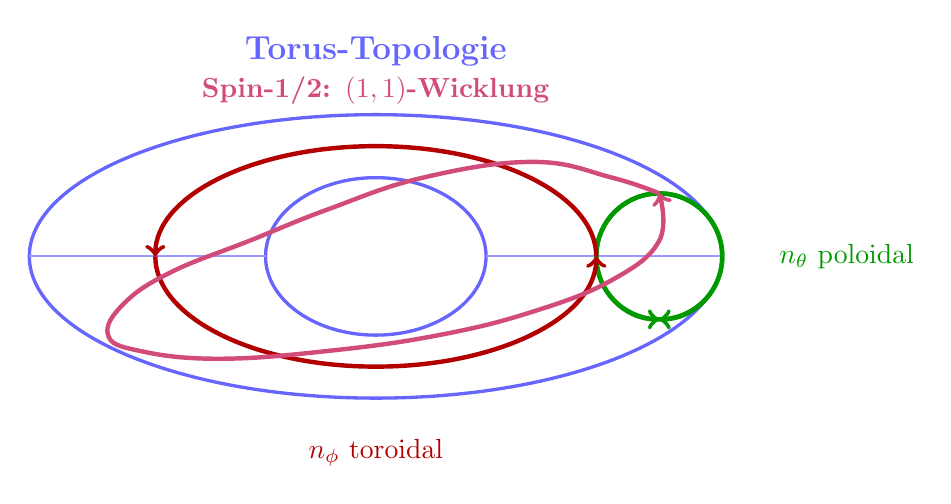
\begin{tikzpicture}[scale=2.0]
		% Torus - äußere Kontur (Draufsicht)
		\draw[very thick, blue!60] (0,0) ellipse (2.2cm and 0.9cm);
		
		% Inneres Loch
		\draw[very thick, blue!60] (0,0) ellipse (0.7cm and 0.5cm);
		
		% Verbindungslinien (optional für 3D-Effekt)
		\draw[thick, blue!40] (-2.2,0) -- (-0.7,0);
		\draw[thick, blue!40] (2.2,0) -- (0.7,0);
		
		% Poloidaler Kreis (kleiner Kreis) - rechts außen, DOPPELT
		\begin{scope}[shift={(1.8,0)}]
			\draw[ultra thick, green!60!black] (0,0) circle (0.4cm);
			\draw[ultra thick, green!60!black, ->] (0,0.4) arc (90:270:0.4cm);
			\draw[ultra thick, green!60!black, ->] (0,0.4) arc (90:-90:0.4cm);
		\end{scope}
		\node[green!60!black, right] at (2.5,0) {$n_\theta$ poloidal};
		
		% Toroidaler Pfad (großer Kreis, um den Mittelpunkt)
		\draw[ultra thick, red!70!black, ->] 
		(1.4,0) arc[start angle=0, end angle=180, x radius=1.4cm, y radius=0.7cm];
		\draw[ultra thick, red!70!black, ->] 
		(-1.4,0) arc[start angle=180, end angle=360, x radius=1.4cm, y radius=0.7cm];
		\node[red!70!black, below] at (0,-1.1) {$n_\phi$ toroidal};
		
		% Spin-1/2 Wicklung (1,1) - einmal um klein, einmal um groß
		\draw[ultra thick, purple!70, ->] 
		plot[smooth, tension=0.7] coordinates {
			(1.8,0.4) (1.5,0.5) (1.0,0.6) (0.3,0.5) (-0.3,0.3) 
			(-0.8,0.1) (-1.3,-0.1) (-1.6,-0.3) (-1.7,-0.5)
			(-1.5,-0.6) (-1.0,-0.65) (-0.3,-0.6) (0.4,-0.5)
			(1.0,-0.35) (1.5,-0.15) (1.8,0.1) (1.8,0.4)
		};
		\node[purple!70, above] at (0,0.9) {\textbf{Spin-1/2: $(1,1)$-Wicklung}};
		
		% Titel
		\node[blue!60, font=\large] at (0,1.3) {\textbf{Torus-Topologie}};
	\end{tikzpicture}
	\caption{Spin-1/2 als topologische Wicklung auf dem Torus (Draufsicht). Der 
		grüne Doppelpfeil zeigt den poloidalen kleinen Kreis ($n_\theta$, Querschnitt 
		des Torus-Schlauchs). Die roten Pfeile zeigen die toroidale Richtung ($n_\phi$, 
		um das zentrale Loch). Der violette Pfad zeigt eine $(1,1)$-Wicklung: einmal 
		um den kleinen Kreis UND einmal um den großen Kreis. Eine 720°-Rotation 
		entspricht zweimaligem Durchlaufen dieser Wicklung.}
	\label{fig:spin_winding}
\end{figure}

\subsection{Häufige Missverständnisse}
\label{subsec:common_misconceptions}

\subsubsection{Kann man die Matrizen wirklich eliminieren?}

\textbf{Antwort: Ja und Nein.}

\begin{itemize}
	\item \textbf{Ja -- fundamental:} Die Physik braucht keine spezifischen 
	4×4-Matrizen. Die Clifford-Algebra ist fundamental.
	
	\item \textbf{Nein -- praktisch:} Für konkrete Berechnungen ist eine Darstellung 
	nötig, und Matrizen sind oft die praktischste Wahl.
\end{itemize}

\textbf{Analogie:} Man kann Vektorphysik ohne Koordinaten formulieren (fundamental), 
aber für Berechnungen wählt man Koordinaten (praktisch).

\subsubsection{Verliert man Information?}

\textbf{Nein!} Die Clifford-Algebra-Formulierung enthält \textbf{genau dieselbe 
	Information}:

\begin{table}[h]
	\centering
	\begin{tabular}{lcc}
		\toprule
		\textbf{Eigenschaft} & \textbf{In Matrizen} & \textbf{In Clifford-Algebra} \\
		\midrule
		Spin-1/2 & In $\gamma$-Struktur & In Clifford-Produkt-Regel \\
		Lorentz-Inv. & Explizit in Matrizen & In $g_{\mu\nu}$-Struktur \\
		Antiteilchen & Neg. Energie-Lösungen & Chiralitäts-Komponenten \\
		Messgrößen & Matrixelemente & Invariante unter Darstellung \\
		\bottomrule
	\end{tabular}
	\caption{Information in beiden Formulierungen identisch}
\end{table}

\subsubsection{Ist dies nur eine Umformulierung?}

\textbf{Nein -- es ist eine konzeptionelle Verschiebung:}

\begin{itemize}
	\item \textbf{Alte Sicht:} ``Elektronen sind Punktteilchen mit mysteriösem 
	intrinsischen Spin, beschrieben durch komplizierte 4×4-Matrizen''
	
	\item \textbf{Neue Sicht:} ``Elektronen sind geometrische Objekte in einer 
	Clifford-strukturierten Raumzeit. Spin ist eine topologische Eigenschaft.''
\end{itemize}

Diese neue Sicht ermöglicht die \textbf{natürliche Integration} in die T0-Theorie:
\begin{itemize}
	\item Fraktale Metrik $\rightarrow$ modifizierte Clifford-Struktur
	\item Torus-Topologie $\rightarrow$ Spin als Wicklungszahl
	\item Zeit-Masse-Dualität $\rightarrow$ dynamische Masse $m(x)$
\end{itemize}

\subsection{Vorbereitung für T0-Integration}
\label{subsec:preparation_t0}

Mit diesem Verständnis können wir nun die T0-spezifischen Modifikationen einführen:

\begin{enumerate}
	\item \textbf{Fraktale Metrik:} $g_{\mu\nu} \rightarrow g_{\mu\nu}^{\text{(frak)}}$ 
	mit $D_f = 3 - \xi$
	
	\item \textbf{Modifizierte Clifford-Regel:}
	\begin{equation}
		\mathbf{e}_\mu^{\text{(frak)}} \mathbf{e}_\nu^{\text{(frak)}} + 
		\mathbf{e}_\nu^{\text{(frak)}} \mathbf{e}_\mu^{\text{(frak)}} = 
		2 g_{\mu\nu}^{\text{(frak)}}
	\end{equation}
	
	\item \textbf{Dynamische Masse:} $m \rightarrow m(x) = 1/(c^2 T(x))$
	
	\item \textbf{Tetrad-Formulierung:} Notwendig für gekrümmte/fraktale Raumzeit
\end{enumerate}

Im nächsten Abschnitt entwickeln wir diese T0-spezifische Formulierung im Detail.

\begin{keypoint}[Kernbotschaft dieses Kapitels]
	Die Dirac-Gleichung ist fundamental eine \textbf{geometrische Gleichung} in der 
	Clifford-Algebra der Raumzeit. Die 4×4-Matrizen sind nützliche 
	Berechnungswerkzeuge, aber nicht die Physik selbst. Diese Erkenntnis ist 
	\textbf{essentiell} für die Integration in die T0-Theorie mit ihrer fraktalen 
	Geometrie und Torus-Topologie.
\end{keypoint}	
	\section{T0-Dirac-Gleichung: Geometrische Form}
	
	\subsection{Clifford-Algebra in fraktaler Raumzeit}
	
	Statt der Standard-Form verwenden wir die Clifford-Algebra-Formulierung:
	\begin{equation}
		\boxed{(i \partial\!\!\!/_{\text{frak}} - m(x))\Psi(x) = 0}
		\label{eq:t0_dirac}
	\end{equation}
	
	wobei:
	\begin{align}
		\partial\!\!\!/_{\text{frak}} &= \mathbf{e}^\mu_a(x) \gamma^a \partial_\mu 
		\quad \text{(tetrad-basiert)} \\
		m(x) &= \frac{1}{c^2 T(x)} \quad \text{(aus Zeit-Masse-Dualität)} \\
		\mathbf{e}^\mu_a(x) &= \text{Tetrad in fraktaler Metrik}
	\end{align}
	
	\subsection{Fraktale Metrik}
	
	Die fraktale Korrektur zur Metrik ist:
	\begin{equation}
		g_{\mu\nu}^{\text{(frak)}}(x) = \eta_{\mu\nu} \cdot \left(1 + \xi \cdot f(x)\right)
		\label{eq:fractal_metric}
	\end{equation}
	
	wobei $f(x)$ eine dimensionslose Funktion der Koordinaten ist, die die fraktale 
	Struktur beschreibt.
	
	\subsection{Tetrad-Formulierung}
	
	Das Tetrad $\mathbf{e}^\mu_a(x)$ verbindet die gekrümmte Raumzeit mit der lokalen 
	Clifford-Algebra:
	\begin{equation}
		g_{\mu\nu}^{\text{(frak)}}(x) = \mathbf{e}^\mu_a(x) \mathbf{e}^\nu_b(x) \eta^{ab}
		\label{eq:tetrad_metric}
	\end{equation}
	
	Die $\gamma^a$ sind die Standard-Clifford-Generatoren im lokalen Lorentz-Frame.
	
	\section{Dynamische Masse}
	
	\subsection{Raumzeit-Abhängigkeit}
	
	Aus der Zeit-Masse-Dualität folgt:
	\begin{equation}
		m(x,t) = \frac{1}{c^2 T(x,t)} = \frac{1}{c^2} \max(\omega(x,t), m_{\text{bg}}(x))
		\label{eq:dynamic_mass}
	\end{equation}
	
	wobei:
	\begin{itemize}
		\item $\omega(x,t)$: Lokale Frequenz/Energie-Dichte
		\item $m_{\text{bg}}(x)$: Hintergrund-Massenfeld
	\end{itemize}
	
	\subsection{Kopplung an Zeitfeld}
	
	Das Zeitfeld $T(x,t)$ ist selbst ein dynamisches Feld mit Lagrange-Dichte:
	\begin{equation}
		\mathcal{L}_T = \frac{1}{2}(\partial_\mu T)(\partial^\mu T) - V(T)
		\label{eq:time_lagrangian}
	\end{equation}
	
	Die Kopplung an Fermionen erfolgt durch die Masse:
	\begin{equation}
		\mathcal{L}_{\text{int}} = \bar{\Psi} m(T(x)) \Psi
		\label{eq:fermion_time_coupling}
	\end{equation}
	
	\section{Spin als Topologie}
	
	\subsection{Wicklungszahlen auf dem Torus}
	
	In der T0-Theorie wird Spin als Wicklungszahl interpretiert:
	\begin{equation}
		\text{Spin-}s \quad \longleftrightarrow \quad 
		\text{Wicklung } (n_\theta, n_\phi) \text{ mit } n_\phi/n_\theta = 2s
		\label{eq:spin_topology}
	\end{equation}
	
	\textbf{Beispiele:}
	\begin{align}
		\text{Spin-}0: &\quad (1, 0) \text{ oder } (0, 1) \\
		\text{Spin-}1/2: &\quad (1, 1) \text{ oder } (2, 1) \\
		\text{Spin-}1: &\quad (1, 2)
	\end{align}
	
	\subsection{720°-Rotation geometrisch}
	
	Die bekannte Eigenschaft von Spin-1/2 Teilchen (720°-Rotation für Identität) 
	folgt aus der Torus-Topologie:
	
	\begin{itemize}
		\item Eine poloidale Wicklung: 360°-Rotation → $-\Psi$
		\item Zwei poloidale Wicklungen: 720°-Rotation → $+\Psi$
	\end{itemize}
	
	Dies ist keine mysteröse Eigenschaft, sondern **reine Topologie**.
	
	\section{Massenproportionale Kopplung}
	
	\subsection{Wechselwirkungslagrangian}
	
	Die Kopplung von Leptonen an das Zeitfeld ist massenproportional:
	\begin{equation}
		\mathcal{L}_{\text{int}} = \xi m_\ell \bar{\Psi}_\ell \Psi_\ell \Delta m(x)
		\label{eq:mass_proportional}
	\end{equation}
	
	wobei $\Delta m(x) = m(x) - m_0$ die Massenfluktuation ist.
	
	\subsection{Konsequenz: Quadratische Skalierung}
	
	Aus dieser massenproportionalen Kopplung folgt für Schleifendiagramme:
	\begin{equation}
		\Delta a_\ell \propto (\xi m_\ell)^2 \cdot \text{(kinematische Faktoren)} \propto m_\ell^2
		\label{eq:quadratic_scaling}
	\end{equation}
	
	Dies führt zur fundamentalen Verhältnisvorhersage:
	\begin{equation}
		\boxed{\frac{\Delta a_{\ell_1}}{\Delta a_{\ell_2}} = \left(\frac{m_{\ell_1}}{m_{\ell_2}}\right)^2}
		\label{eq:ratio_prediction}
	\end{equation}
	
	\section{Verhältnisse vs. Absolute Werte}
	
	\subsection{Was die T0-Dirac-Gleichung vorhersagt}
	
	\textbf{Fundamentale Vorhersagen (parameterfrei):}
	\begin{itemize}
		\item Verhältnis: $a_\tau/a_\mu = (m_\tau/m_\mu)^2 \approx 283$
		\item Struktur: $\Delta a \propto m^2$ (quadratische Skalierung)
		\item Topologie: Spin-1/2 als Wicklungszahl
	\end{itemize}
	
	\textbf{Nicht vorhersagbar (phänomenologisch):}
	\begin{itemize}
		\item Absolute Werte: $a_\mu = 37.5 \times 10^{-11}$ (braucht Normierung)

	\end{itemize}
	
	\subsection{Warum nur Verhältnisse?}
	
	Die vollständige Berechnung absoluter Werte erfordert:
	\begin{enumerate}
		\item Lösung der Zeitfeld-Dynamik in fraktaler Raumzeit (zu komplex)
		\item Schleifenintegrale in nicht-ganzzahliger Dimension (offen)
		\item Renormierung bei $D_f = 3 - \xi$ (nicht vollständig entwickelt)
		\item Rekursive Kopplung aller Felder (nicht-perturbativ)
	\end{enumerate}
	
	Dies ist analog zu QCD im Standardmodell: Fundamentale Lagrange-Dichte ist klar, 
	aber hadronische Beiträge nicht ab initio berechenbar.
	
	\section{Natürliche vs. SI-Einheiten}
	
	\subsection{In natürlichen Einheiten}
	
	In natürlichen Einheiten ($\hbar = c = 1$, $\alpha = 1$) verschwindet $\alpha$ 
	aus allen Formeln:
	
	\begin{equation}
		\tilde{a}_\ell = \tilde{C} \cdot \xi \cdot \tilde{m}_\ell^2
		\label{eq:natural_units}
	\end{equation}
	
	Das Verhältnis ist:
	\begin{equation}
		\frac{\tilde{a}_\tau}{\tilde{a}_\mu} = \left(\frac{\tilde{m}_\tau}{\tilde{m}_\mu}\right)^2
	\end{equation}
	
	**Identisch mit SI-Version** – Verhältnisse sind invariant!
	
	\subsection{Transformation zu SI}
	
	Die Transformation zu SI-Einheiten führt $\alpha$ ein:
	\begin{equation}
		a_\ell[\text{SI}] = \text{(Umrechnungsfaktor mit } \alpha\text{)} \times \tilde{a}_\ell
	\end{equation}
	
	Aber das **Verhältnis bleibt unverändert**:
	\begin{equation}
		\frac{a_\tau[\text{SI}]}{a_\mu[\text{SI}]} = \frac{\tilde{a}_\tau}{\tilde{a}_\mu} = 
		\left(\frac{m_\tau}{m_\mu}\right)^2
	\end{equation}
	
	\section{Experimentelle Tests}
	
	\subsection{Belle II: Kritischer Test (2027-2028)}
	
	Die fundamentale Vorhersage:
	\begin{equation}
		\frac{a_\tau}{a_\mu} = \left(\frac{1776.86}{105.658}\right)^2 = 282.8
	\end{equation}
	
	ist direkt testbar bei Belle II.
	
	\textbf{Mögliche Ergebnisse:}
	\begin{itemize}
		\item \textbf{Bestätigung}: Starke Evidenz für massenproportionale Kopplung
		\item \textbf{Abweichung}: Modifikation der Kopplungsstruktur nötig
		\item \textbf{Null-Ergebnis}: T0-Beiträge unterdrückt oder falsch
	\end{itemize}
	
	\subsection{Weitere Tests}
	
	\begin{table}[h]
		\centering
		\begin{tabular}{lcc}
			\toprule
			\textbf{Test} & \textbf{T0-Vorhersage} & \textbf{Status} \\
			\midrule
			$a_\tau/a_\mu$ & $(m_\tau/m_\mu)^2 = 283$ & Belle II 2027-28 \\
			$m_\tau/m_\mu$ & $\approx 16.8$ (aus Torus) & Bestätigt ✓ \\
			Spin-Statistik & Aus Topologie & Bestätigt ✓ \\
			Fraktale Dämpfung & $\propto e^{-\xi n^2}$ & Rydberg-Atome \\
			\bottomrule
		\end{tabular}
		\caption{Experimentelle Tests der T0-Dirac-Formulierung}
	\end{table}
	
	\section{Vergleich mit Standard-Formulierung}
	
	\begin{table}[h]
		\centering
		\begin{tabular}{lcc}
			\toprule
			\textbf{Aspekt} & \textbf{Standard-Dirac} & \textbf{T0-Dirac} \\
			\midrule
			Masse & Konstant $m$ & Dynamisch $m(x,t)$ \\
			Metrik & Minkowski $\eta_{\mu\nu}$ & Fraktal $g_{\mu\nu}^{\text{(frak)}}$ \\
			Spin & Matrixeigenschaft & Topologische Wicklung \\
			Dimension & $D = 4$ & $D_f = 3 - \xi$ in Raum \\
			Topologie & Keine & Torus $(n_\theta, n_\phi)$ \\
			Kopplung & Ad-hoc & Zeit-Masse-Dualität \\
			Vorhersagen & Qualitativ & Verhältnisse testbar \\
			\bottomrule
		\end{tabular}
		\caption{Standard vs. T0 Dirac-Formulierung}
	\end{table}
	
	\section{Grenzen und offene Fragen}
	
	\subsection{Was funktioniert}
	
	\begin{itemize}
		\item ✓ Clifford-Algebra-Struktur klar definiert
		\item ✓ Spin als Topologie interpretierbar
		\item ✓ Verhältnisvorhersagen parameterfrei
		\item ✓ Belle II Test möglich
	\end{itemize}

	\subsection{Ehrlichkeit über Grenzen}
	
	Wie im Standardmodell (hadronische Beiträge) gibt es Bereiche, wo die fundamentale 
	Theorie klar ist, aber explizite Berechnungen zu komplex sind. Dies ist **kein 
	Fehler der Theorie**, sondern eine realistische Einschätzung der mathematischen 
	Herausforderungen.
	
\section*{Literaturverzeichnis und Weiterführende Literatur}

\begin{thebibliography}{9}
	
	\bibitem{T0Foundation}
	J. Pascher,
	\textit{Die T0-Grundlage: Zeit-Masse-Dualität und fraktale Geometrie},
	T0-Time-Mass-Duality Repository,
	2026.
	
	\bibitem{XiNarrative}
	J. Pascher,
	\textit{Die Xi-Erzählung: Von einer einzigen Zahl zur Feinstrukturkonstanten},
	FFGFT\_Narrative\_Master\_De.pdf,
	2025.
	
	\bibitem{CliffordGeometricAlgebra}
	D. Hestenes,
	\textit{Raum-Zeit-Algebra},
	Gordon and Breach, 1966.
	Liefert die mathematische Grundlage für geometrische Clifford-Algebra-Formulierungen.
	
	\bibitem{CliffordSpinors}
	P. Lounesto,
	\textit{Clifford-Algebren und Spinoren},
	Cambridge University Press, 2001.
	Umfassende Behandlung von Clifford-Algebren mit Anwendungen auf Spinoren.
	
	\bibitem{DiracOriginal}
	P. A. M. Dirac,
	\textit{Die Quantentheorie des Elektrons},
	Proc. R. Soc. Lond. A, 117, 610–624, 1928.
	Das Originalpapier zur Einführung der Dirac-Gleichung.
	
	\bibitem{TorusTopologySpin}
	J. Williamson und M. B. van der Mark,
	\textit{Ist das Elektron ein Photon mit toroidaler Topologie?},
	Annales de la Fondation Louis de Broglie, 22, 133–167, 1997.
	\href{https://fondationlouisdebroglie.org/IMG/pdf/22_2_133.pdf}{[PDF]}
	
	\bibitem{BelleIITauG2}
	Belle II-Kollaboration,
	\textit{Aussichten für die Messung des anomalen magnetischen Moments des Tau-Leptons bei Belle II},
	Belle II Note 0123, 2024.
	\href{https://www.belle2.org}{[Belle II Website]}
	
	\bibitem{FermilabMuonG2}
	Muon g-2-Kollaboration,
	\textit{Messung des anomalen magnetischen Moments des positiven Myons auf 0.20 ppm},
	Phys. Rev. Lett. 131, 161802, 2023.
	Aktuelle Ergebnisse von Fermilab.
	
	\bibitem{GeometricTopologyPhysics}
	M. Nakahara,
	\textit{Geometrie, Topologie und Physik},
	IOP Publishing, 2003.
	Hervorragende Ressource für Tetraden-Formalismus und Differentialgeometrie in der Physik.
	
	\bibitem{FractalGeometry}
	K. Falconer,
	\textit{Fraktale Geometrie: Mathematische Grundlagen und Anwendungen},
	Wiley, 2014.
	Standardreferenz für fraktale Geometrie und Hausdorff-Dimensionen.
	
	\bibitem{TimeMassDualityDerivation}
	J. Pascher,
	\textit{Herleitung der Zeit-Masse-Dualität aus den Planck-Beziehungen},
	T0\_xi\_ursprung.pdf,
	2025.
	
	\bibitem{T0DiracSimplified}
	J. Pascher,
	\textit{Dirac-Gleichung in der T0-Theorie: Geometrische Clifford-Algebra-Formulierung},
	Dokument 050\_dirac\_geometrisch,
	2026.

\end{thebibliography}
	